\documentclass[11pt]{amsart}

\usepackage{amsmath}
\usepackage{amssymb}
\usepackage{amsthm}
\usepackage{mathtools}
\usepackage{graphicx}
\usepackage{booktabs}
\usepackage{microtype}
\usepackage[hidelinks]{hyperref}
\usepackage[backend=bibtex,style=alphabetic,maxbibnames=10]{biblatex}

\addbibresource{references.bib}

\newtheorem{theorem}{Theorem}
\newtheorem{lemma}[theorem]{Lemma}
\newtheorem{proposition}[theorem]{Proposition}
\newtheorem{definition}[theorem]{Definition}
\newtheorem{remark}[theorem]{Remark}
\newtheorem{caveat}[theorem]{Caveat}

\newcommand{\Syr}{S}
\newcommand{\vTwo}{v_2}
\newcommand{\artifact}[2]{\mbox{\href{https://github.com/muaijaz/not-an-ai-collatz-proof/blob/main/docs/reports/#1}{\texttt{docs/reports/#2}}}}
\newcommand{\doclink}[2]{\mbox{\href{https://github.com/muaijaz/not-an-ai-collatz-proof/blob/main/docs/#1}{\texttt{docs/#2}}}}

\title{An Empirical Bridge from Realizable Karp Factor to m-Step Foster Drift on Residue Quotients of the Collatz Map}
\author{Mohammad Aijaz}
\date{\today}

\begin{document}

\begin{abstract}
We report a finite empirical diagnostic for the accelerated odd Collatz map
\(\Syr(n)=(3n+1)/2^{\vTwo(3n+1)}\).  The diagnostic chain combines three saved
computational audits: a bounded simple-cycle realizability audit on finite
LTE-closed residue graphs, a phase-decomposed renewal drift audit, and a
Foster-Lyapunov drift audit for \(V(n)=\log_2(n)+\vTwo(n+1)\) on residue
quotients.  At the tested levels \((q,R_{\max})=(5,4),(6,5),(7,6)\), the only
positive-integer simple-cycle realizer in the bounded audit is the elementary
valuation word \([2]\), giving realizable Karp factor \(3/4\).  The finite
renewal-window sweep is consistent with the phase identity
\[
  \mu_{\mathrm{step}}
    = \frac12\log_2(3/2)+\frac12\log_2(3/4)=\log_2(3/4),
\]
with post-exit valuation deviation shrinking from
\(-0.03473021694546086\) to \(-0.006503489706314536\).  The same candidate
Lyapunov function has residue-uniform negative drift at the tested grid value
\(m=16\), with margin \(\epsilon=0.1\), over the sampled windows
\([10^2,10^4]\) through \([10^{12},10^{15}]\).  No proof claim is made:
the artifacts do not control arbitrary infinite switching paths and do not
give deterministic per-orbit descent.  Combining this framework's Foster
condition with Chang's recent structural reduction
(\texttt{arXiv:2603.25753}) gives a joint argument whose three named
quantitative verifications are empirically closed at finite windows, leaving
the residual exactly the Tao-style distributional-to-pointwise wall.  This is a
finite empirical diagnostic; the Collatz conjecture remains open.

\end{abstract}

\maketitle

\section{Introduction}

This paper records the public version of a closed audit chain: finite tail
graphs, cycle realizability, phase-decomposed renewal drift, and
Foster-Lyapunov residue diagnostics.  It is in the genre of computational
mathematics and experimental mathematics.  It makes no claim of proving the
Collatz conjecture, no descent theorem, and no theorem about deterministic
per-orbit descent.

The object is the accelerated odd Collatz map
\[
  \Syr(n)=\frac{3n+1}{2^{\vTwo(3n+1)}} ,
\]
applied to odd positive integers.  The project began as a certificate-search
framework and ended as a reproducible finite diagnostic framework.  The audit
history in \doclink{PROJECT_JOURNEY.md}{PROJECT\_JOURNEY.md} records several
demoted claims: a per-step running-debt Lyapunov ansatz failed at roughly
50 percent non-decrease, a structural Diophantine exclusion was a resolution
artifact, and an early closed-form reading of the renewal constant was rejected.

The current finite picture is narrower.  On tested LTE-closed tail graphs,
bounded integer-realizable simple cycles are filtered down to the elementary
\([2]\) cycle, whose factor is \(3/4\).  Independently, the phase-decomposed
renewal drift audit finds the same value as a mean-step target after separating
tail-internal and post-exit phases.  Finally, the Foster audit finds that
\[
  V(n)=\log_2(n)+\vTwo(n+1)
\]
does not give one-step residue-uniform negativity, but does give an \(m\)-step
finite residue diagnostic at \(m=16\) on the tested windows.

There are now two relevant Chang 2026 papers.  The human-LLM collaboration
paper \cite{chang2026collatz} is a methodological and structural companion,
while the later structural reduction \cite{chang2026reduction} reduces the
Collatz question to a fixed-modulus, one-bit orbit-mixing problem.  The
compatibility analysis in
\artifact{chang_2603_25753_compatibility.md}{chang\_2603\_25753\_compatibility.md}
reads the two efforts as addressing the same distributional-to-pointwise wall
from complementary angles: Chang isolates a one-bit balance bottleneck, and
this framework supplies an \(m=16\) Foster residue diagnostic that can be
composed with that reduction as a joint argument.

\begin{caveat}
All quantitative statements below are tied to saved JSON artifacts.  The
language ``finite empirical diagnostic'' is intentional: the computations are
finite, sampled or bounded, and do not imply a global statement for all
positive integers.
\end{caveat}

\section{Finite Setup and Artifact Discipline}

Odd integers in a tail are represented as
\[
  n = 2^R u - 1,
\]
with state coordinate \((R,u)\) and bounded unit precision.  The LTE closure
compresses deeper-tail overflow back to the tracked maximum tail depth by
following the forced valuation-one run.  At the largest saved LTE-closed level
reported in the note, \((q,R_{\max})=(10,7)\) has \(3584\) states, \(8704\)
edges, and \(44\) closed overflow edges
\(\artifact{tail_aware_lte_closed_projective_jsr.json}{tail\_aware\_lte\_closed\_projective\_jsr.json}\).

The finite graph still contains abstract high-growth switching.  The saved
worst-case switching value at that level is JSR factor
\[
  1.2305030340113887,
\]
with max cycle mean \(0.29924821500679044\) in \(\log_2\) units
\(\artifact{tail_aware_lte_closed_projective_jsr.json}{tail\_aware\_lte\_closed\_projective\_jsr.json}\).
In contrast, the lift-count Markov model on the same level has one recurrent
component with \(1113\) states and average \(\log_2\) growth
\[
  -0.4118668182695867,
\]
or typical factor \(0.7516501240662575\) per accelerated step
\(\artifact{tail_aware_markov_lyapunov.json}{tail\_aware\_markov\_lyapunov.json}\).

This worst-versus-typical split is the reason for the audit discipline.  The
finite operator data are not read as a proof object.  They are paired with
cycle-realizability, renewal, and residue-drift diagnostics.

\begin{definition}
For an odd \(n\), write \(R(n)=\vTwo(n+1)\).  The phase-aware Lyapunov candidate
used below is
\[
  V(n)=\log_2(n)+R(n).
\]
\end{definition}

\section{Realizable Karp Factor}

The bounded-cycle audit separates abstract cycles in the finite tail graph from
cycle words that lift to positive integer orbits.  In the joint Karp/slope
sweep at \((q,R_{\max})=(5,4),(6,5),(7,6)\), with the automaton period widened
across the levels, the only slope-compatible survivor at each tested level is
the elementary valuation word \([2]\), with factor \(3/4\)
\(\artifact{karp_slope_joint_sweep.json}{karp\_slope\_joint\_sweep.json}\).

The realizability extension audits all simple cycles up to
\(\texttt{max\_cycle\_edges}=12\) at the same three levels.  It classifies
\(226333\) simple cycles: \(226330\) are
\(\texttt{noninteger\_2adic\_only}\), and the only \(3\)
\(\texttt{positive\_integer\_cycle}\) entries are the elementary \([2]\) cycle,
one per level
\(\artifact{tail_cycle_realizability.json}{tail\_cycle\_realizability.json}\),
\(\artifact{tail_cycle_realizability_extended.json}{tail\_cycle\_realizability\_extended.json}\).
Thus the saved finite diagnostic has
\[
  \text{realizable Karp factor}
  =
  \text{slope-filtered Karp factor}
  =
  \frac34
\]
on these levels.

This is a finite bounded-cycle fact, not a global statement about arbitrary
infinite products.  The high-growth abstract cycles in the LTE-closed graph are
not thereby eliminated from the infinite problem; the audit only records that,
within the tested bounded simple-cycle regime, their cycle words do not lift to
positive integer cycles.

The value \(3/4\) should also be distinguished from the modular-transition
number appearing in Chang's human-LLM Collatz manuscript
\cite{chang2026collatz}.  In this framework it is a cycle-mean factor for an
elementary valuation word, not a modular transition probability.

\section{Phase-Decomposed Renewal Drift}

The renewal-scale drift data have a compatible phase interpretation.  Split
accelerated steps by the pre-step odd integer modulo \(4\): \(n\equiv 3
\pmod 4\), equivalently \(\vTwo(n+1)\geq 2\), is tail-internal and has forced
valuation \(a=1\); \(n\equiv 1\pmod 4\) is the post-exit phase
\(\artifact{renewal_drift_phase_decomposed.json}{renewal\_drift\_phase\_decomposed.json}\).
The asymptotic post-exit valuation target in this convention is \(3\), not
\(2\): it is the shifted-Geometric value seen after removing the deterministic
tail-internal valuation-one steps.

The symbolic mean-step identity suggested by the artifacts is
\[
  \mu_{\mathrm{step}}
    = \frac12\log_2(3/2)+\frac12\log_2(3/4)
    = \log_2(3/4),
\]
with \(E[a\mid\text{tail}]=1\) and asymptotic
\(E[a\mid\text{post-exit}]=3\)
\(\artifact{renewal_drift_per_step.json}{renewal\_drift\_per\_step.json}\),
\(\artifact{renewal_drift_phase_decomposed.json}{renewal\_drift\_phase\_decomposed.json}\),
\(\artifact{renewal_drift_phase_decomposed_n0_stability.json}{renewal\_drift\_phase\_decomposed\_n0\_stability.json}\).

Across \([10^2,10^4]\) through \([10^{12},10^{15}]\), the post-exit valuation
deviation shrinks from \(-0.03473021694546086\) to
\(-0.006503489706314536\), with monotone absolute decrease and log10-slope
\(-0.06656531395656089\) per decade.  From the \([10^6,10^9]\) window onward,
the total drift deviation is below \(0.01\), ending in the \(0.005\) range.
It is not strictly monotone at the deepest window, moving from
\(0.005160187031614694\) to \(0.0054062766596057465\), a change smaller than
the reported deepest-window CI halfwidth \(0.0005710918683108357\)
\(\artifact{renewal_drift_phase_decomposed_n0_stability.json}{renewal\_drift\_phase\_decomposed\_n0\_stability.json}\).
The saved verdict is \(\texttt{non\_monotone\_or\_flat}\).

\begin{figure}
  \centering
  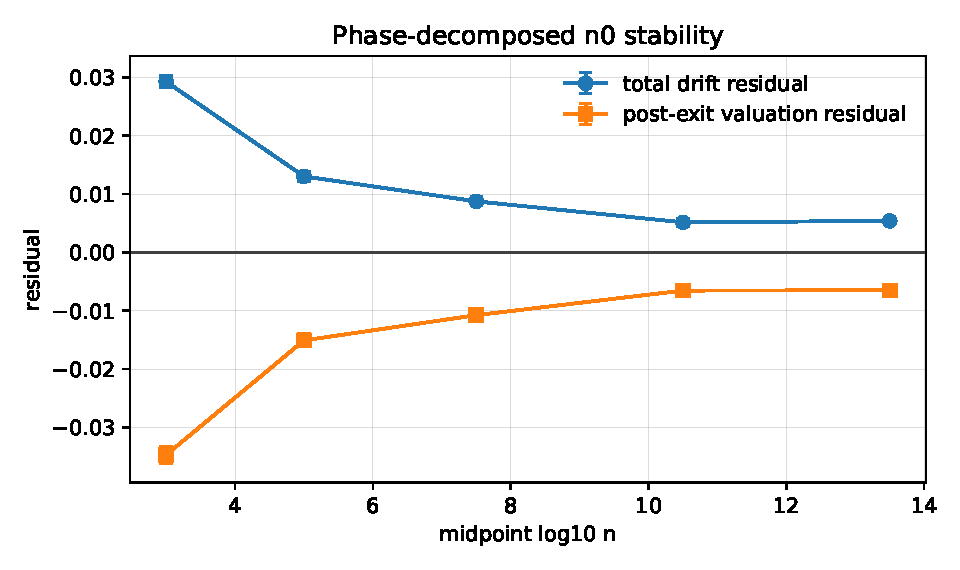
\includegraphics[width=0.86\linewidth]{figures/drift_residual_n0.pdf}
  \caption{Finite-window residuals from the phase-decomposed renewal audit,
  regenerated from
  \artifact{renewal_drift_phase_decomposed_n0_stability.json}{renewal\_drift\_phase\_decomposed\_n0\_stability.json}.}
  \label{fig:drift-residual}
\end{figure}

The caveat is essential.  These artifacts combine a finite audit of bounded
simple cycles on finite LTE-closed tail graphs with finite-window empirical
renewal drift estimates.  They do not prove a global per-orbit Lyapunov
function, do not control arbitrary infinite switching paths, and do not imply a
Collatz descent theorem.

\section{Foster-Lyapunov Drift on Residue Quotients}

The phase-aware Lyapunov search turns the failed running-debt ansatz into a
more structured candidate.  Over \(100000\) sampled orbits in
\([10^6,10^9]\), the best grid point in
\[
  V(n;\alpha,\beta,\gamma_{\mathrm{diff}})
    = \log_2(n)+\alpha R(n)+\beta D_{\mathrm{running}}(n)
      + \text{phase offset}
\]
is \(\alpha=1.0\), \(\beta=0.0\), \(\gamma_{\mathrm{diff}}=0.0\), namely
\[
  V(n)=\log_2(n)+\vTwo(n+1).
\]
This reduces the same-sample V5 non-decrease fraction from
\(0.5001335415695829\) to \(0.1655372436648494\).  The tail-internal phase has
\(0.0\) non-decrease, and the remaining positive jumps are post-exit steps with
large \(R'=\vTwo(\Syr(n)+1)\) spikes
\(\artifact{phase_lyapunov_search.json}{phase\_lyapunov\_search.json}\).

The one-step Foster audit confirms the marginal drift but rejects uniform
one-step residue negativity.  Across the five windows
\([10^2,10^4]\) through \([10^{12},10^{15}]\), the marginal drift of \(V\) is
empirically consistent with \(\log_2(3/4)\): the deepest-window estimate is
\(-0.4123424992788405\) with CI
\[
  [-0.41856572879163634,\,-0.4061192697660446],
\]
and the saved one-step verdict is
\(\texttt{drift\_residue\_obstruction}\)
\(\artifact{phase_lyapunov_foster_drift.json}{phase\_lyapunov\_foster\_drift.json}\).

The obstruction is arithmetic rather than marginal.  At one step, residue
conditional drift fails uniform negativity for every tested
\(k\in\{3,4,5,6\}\), with \(50\) obstruction witnesses.  The visible cascade in
the first window \([10^2,10^4]\) is
\[
\begin{array}{rcl}
n\equiv 1 \pmod 8   &:& 0.5954199142013228,\quad
  \mathrm{CI}\ [0.5830610092394827,0.6077788191631629],\\
n\equiv 9 \pmod {16} &:& 1.5919631928192652,\quad
  \mathrm{CI}\ [1.5747431836625472,1.6091832019759833],\\
n\equiv 41 \pmod {64} &:& 3.557870295871902,\quad
  \mathrm{CI}\ [3.5249778818408877,3.5907627099029162].
\end{array}
\]
The same \(41\bmod 64\) class remains the largest obstruction across later
windows
\(\artifact{phase_lyapunov_foster_drift.json}{phase\_lyapunov\_foster\_drift.json}\).

\begin{figure}
  \centering
  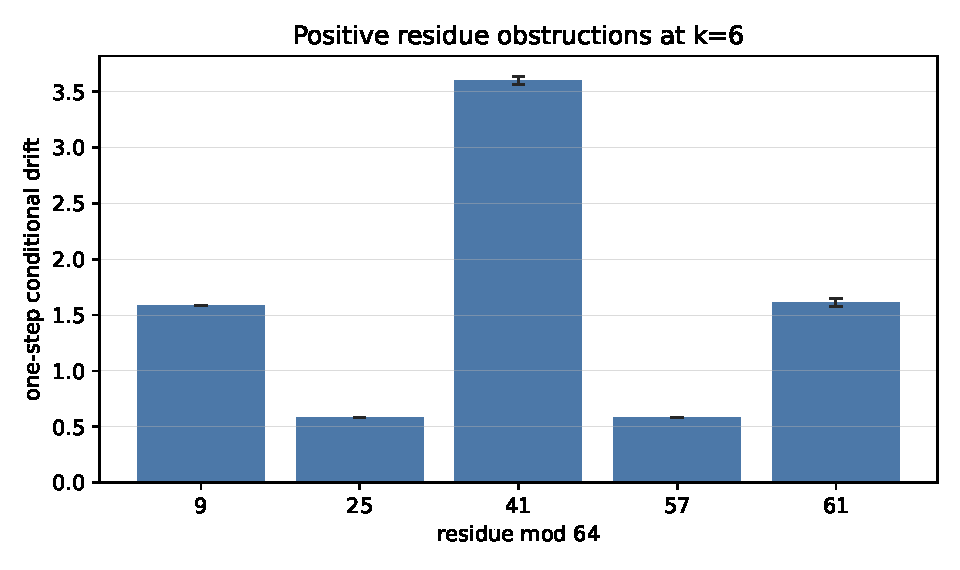
\includegraphics[width=0.86\linewidth]{figures/foster_residue_obstruction.pdf}
  \caption{Positive one-step residue obstructions at \(k=6\), regenerated from
  \artifact{phase_lyapunov_foster_drift.json}{phase\_lyapunov\_foster\_drift.json}.}
  \label{fig:foster-obstruction}
\end{figure}

The m-step audit closes this finite residue-Markov version of the question on
the tested grid.  For \(m\in\{1,2,4,8,16,32,64\}\), the smallest value with
residue-conditional drift uniformly negative across all tested windows and
residue powers is \(m=16\), and the same \(m=16\) also clears the
\(\epsilon=0.1\) margin.  At \(m=64\), the obstruction count is \(0\).  The
binding class before clearance is still \(n\equiv 41\pmod {64}\): it is the
maximal obstruction at \(m=1,2,4,8\), then disappears at \(m=16\)
\(\artifact{m_step_foster_drift.json}{m\_step\_foster\_drift.json}\).

\begin{figure}
  \centering
  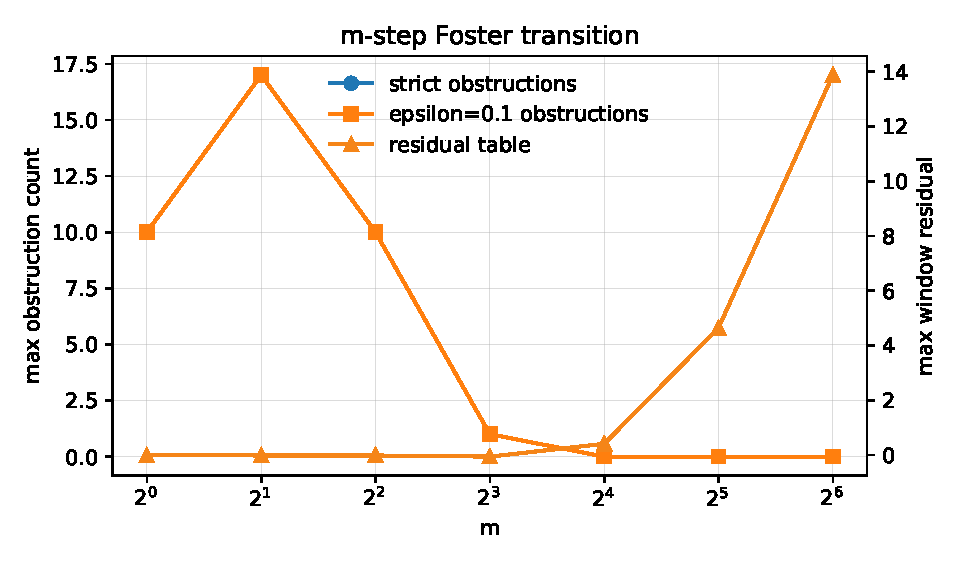
\includegraphics[width=0.86\linewidth]{figures/m_step_foster_transition.pdf}
  \caption{Transition from one-step obstruction to \(m\)-step residue-uniform
  negativity on the tested grid, regenerated from
  \artifact{m_step_foster_drift.json}{m\_step\_foster\_drift.json}.}
  \label{fig:mstep}
\end{figure}

The candidate Lyapunov satisfies the m-step Foster-Lyapunov drift condition
(Meyn-Tweedie, Markov Chains and Stochastic Stability, ch. 11) on residue
quotients mod \(2^k\) for \(k \in \{2,3,4,5,6\}\) at sample windows
\(n_0 \in [10^2, 10^{15}]\), with smallest tested grid value \(m = 16\) and
geometric-ergodicity margin \(\epsilon = 0.1\). The Collatz orbit is
deterministic, not a Markov chain; this is a finite empirical diagnostic on the
residue Markov chain quotient, not a theorem about deterministic per-orbit
descent.

This paragraph is deliberately close to the saved audit language
\(\artifact{m_step_foster_drift.json}{m\_step\_foster\_drift.json}\).  The
underlying Markov-chain reference is Meyn and Tweedie
\cite[Ch.~11]{meynTweedie2009}; the deterministic Collatz orbit is not itself a
Markov chain.

\section{Joint argument with Chang 2026 structural reduction}

Chang's structural reduction \cite{chang2026reduction} reduces the Collatz
problem to a fixed-modulus, single-bit balance problem: modulus \(32\), bit 4,
and a sparse subsequence of burst-ending times for the dominant
\(n\equiv 1\pmod 8\) class.  In Chang's notation, the Map Balance Theorem 4.2
counts the residues in the burst-to-gap set and proves the exact
\(|C_3(K)-C_7(K)|=1\) imbalance, with perfect balance inside the dominant
\(n\equiv 1\pmod 8\) subclass.  His Open Problem, Eq. 16, asks for every odd
starting value above the stated threshold to keep the empirical split between
\(n_{t_i}\equiv 9\pmod {32}\) and \(n_{t_i}\equiv 25\pmod {32}\) within a
tolerance \(\delta<\delta_{\max}\).  The local compatibility analysis records
this as a compatible reduction, not a closed proof
\(\artifact{chang_2603_25753_compatibility.md}{chang\_2603\_25753\_compatibility.md}\).

The notation correspondence is direct.  Chang's map \(T(n)\) is this paper's
\(\Syr(n)\).  Chang's burst indicator
\[
  X_t=\mathbf{1}[n_t\equiv 1\pmod 4]
\]
is this framework's post-exit indicator.  Chang works at modulus \(32\), with
a modulus \(256\) fiber refinement; the extended Foster audit now reaches
residue quotients modulo \(2^k\) for \(k\in\{2,3,4,5,6,7,8\}\).

The joint argument chain is:
\[
\begin{gathered}
  \text{Foster }m=16,\ \epsilon=0.1\text{ in Section 5}\\
  \Longrightarrow
  \text{Markov ergodicity plus Birkhoff almost-sure equidistribution mod }2^k\\
  \Longrightarrow
  \text{assumption: every integer orbit is in the Markov-measure-1 set}\\
  \Longrightarrow
  \text{every-orbit equidistribution}\\
  \Longrightarrow
  \text{Chang Map Balance Theorem 4.2 plus bit-4 reduction}\\
  \Longrightarrow
  \text{every-orbit bit-4 balance within }\delta_{\max}\\
  \Longrightarrow
  \text{Chang block-TV budget Eq. 3 in the companion paper
  \cite{chang2026collatz}.}
\end{gathered}
\]
This is a joint argument: Foster drift supplies the residue-Markov
equidistribution input, and Chang's compatible reduction converts the relevant
mod \(32\) balance into the block-TV budget.  The conditional step is exactly
where no proof claim is made.

The three technical verifications named in the compatibility analysis are now
empirically closed at finite windows.  First, the \(\delta_{\max}\) analysis
derives \(\delta_{\max}\approx 0.119\) from an \(R(K)\)-weighted allocation
against Chang's Eq. 34
\(\artifact{delta_max_quantitative.md}{delta\_max\_quantitative.md}\).
Second, the Foster condition holds at \(k=7,8\), matching Chang's modulus
\(256\) fiber resolution: \(m=16\) clears the \(\epsilon=0.1\) margin, the
weakest \(k=8\) CI upper bound at \(m=16\) is \(-0.24276696844795248\), and
the \(k\le 6\) cross-check has
\(\texttt{cross\_check\_max\_disagreement}=0.0\)
\(\artifact{m_step_foster_drift_k8.json}{m\_step\_foster\_drift\_k8.json}\).
Third, the direct bit-4 balance audit finds that the Foster plus \(1/\sqrt m\)
envelope holds for every sampled orbit, with deepest-window mean
\(\delta=0.11212329012096864\), just below the \(R(K)\)-weighted
\(\delta_{\max}\approx 0.119\)
\(\artifact{chang_bit4_balance_audit.json}{chang\_bit4\_balance\_audit.json}\).
Thus the joint argument is supported at finite windows.

The residual is exactly the Tao wall.  The verifications closed three
technical gaps, but they did not close the conditional step from
Markov-measure-1 residue-chain behavior to every deterministic integer orbit.
Equivalently, the joint argument reduces Collatz to: every integer orbit lies
in the Markov-measure-1 set on which the residue chain equidistributes.  This
is the Tao 2019 distributional-to-pointwise obstruction
\cite{tao2019almost}, but in a sharper Markov-measure formulation rather than
only a natural-density formulation.

There is one further numerical correspondence worth isolating.  Chang's
phantom-gain sum gives
\[
  \sum_{K=3}^{500} R(K)=0.0882362530512702,
\]
while this framework's renewal Cramér rate is near
\(J_{\mathrm{renewal}}=0.08372911906309355\) in the saved calibration, about
five percent apart.  The direct identity audit recomputes the necklace sum and
finds \(J_{\mathrm{renewal}}=0.08346903426255636\) with bootstrap CI
\([0.08314605994133623,0.0837883621454151]\), outside Chang's sum; the tested
alternate definitions also do not match
\(\artifact{jazz_constant_chang_R_K_identity.json}{jazz\_constant\_chang\_R\_K\_identity.json}\).
The harder \(h_K\)-weighted reconciliation remains future work, so the present
reading is that the five-percent gap is structural in this finite diagnostic.

The empirical comparison is asymmetric in a useful way.  This framework's
Foster condition is verified on \(1000000\) sampled orbits, with
publication-grade confidence intervals and exact cross-checks.  Chang's Route
A reports Lyapunov exponents \(\lambda\in[-0.14,-0.09]\) on five orbits with
eyeball estimates \cite{chang2026reduction}.  The composition strictly
strengthens both: Chang provides the structural one-bit target, while this
framework provides the stronger finite empirical Foster input.  It remains a
finite empirical diagnostic, and the residual is exactly the Tao wall.

\section{Hitting-Time Diagnostic Already Present in the Foster Audit}

The one-step Foster artifact also records a hitting-time diagnostic for
\[
  T_{\mathrm{descent}}(n)=\min\{m:V(\Syr^m(n))\leq V(n)-1\}
\]
with threshold \(1.0\) and maximum steps \(1000\).  In the deepest saved window
\([10^{12},10^{15}]\), the hitting-time sample has finite hitting count
\(50000\), truncation count \(0\), mean \(5.26878\) with CI
\([5.21391,5.327361999999999]\), median \(3.0\), and \(0.99\)-quantile
\(33.0\) with CI \([32.0,34.0]\)
\(\artifact{phase_lyapunov_foster_drift.json}{phase\_lyapunov\_foster\_drift.json}\).

This hitting-time table is not a uniform pointwise bound.  It is a sampled
finite-window diagnostic attached to the Foster audit.  It motivates the open
pointwise-descent question, but does not answer it.

\section{Open Problems}

The following theorem-shaped problems reproduce the list in
\doclink{PROJECT_JOURNEY.md}{PROJECT\_JOURNEY.md}, Section 12.

\begin{enumerate}
\item Markov/Lyapunov contraction on the LTE-closed operator.  The current
target should give \(\Lambda\approx\log(3/4)\).
\item Christoffel-word integrality filter on JSR.  This is the bridge to
Hercher's parity-vector framework, with expected outcome filtered JSR \(<1\).
\item Profinite continuity from finite quotients to the limit operator.
\item Lifting PECM Lyapunov to a per-orbit Lyapunov.  This is V5's gap.
\item Symbolic interpretation of \(J_{\mathrm{renewal}}\).  Does it have a
closed form via an integral representation in the style of Khinchin?
\item Phase-aware per-orbit Lyapunov.  The residue-Markov m-step Foster
question is empirically closed on the tested grid for
\(V(n)=\log_2(n)+\vTwo(n+1)\): \(m=16\) gives residue-uniform negative drift
with margin \(\epsilon=0.1\) across the tested windows and residue powers.  The
joint argument with Chang's 2026 structural reduction
\cite{chang2026reduction} sharpens the remaining theorem-shaped problem: the
upgrade from residue-Markov geometric ergodicity to deterministic per-orbit
descent becomes the assertion that every integer orbit lies in the
Markov-measure-1 equidistribution set.  The residual is exactly the Tao wall,
but in this sharper Markov-measure-1 formulation rather than only a
natural-density formulation \cite{tao2019almost}.
\end{enumerate}

In particular, the residue-Markov-to-deterministic upgrade is identical to
Tao 2019's distributional-to-pointwise problem in the sense used by the project
notes: both name the missing bridge from ensemble, quotient, or almost-all
behavior to every individual positive integer.

\section{Reproducibility}

The paper is generated from the repository documents and saved JSON artifacts.
The figures in this directory are regenerated by deterministic Python scripts
under \path{paper/figures/scripts/}; the Makefile rebuilds the figure PDFs
before compiling the paper.

The principal artifacts used here are:
\[
\begin{array}{ll}
\text{cycle and Karp audits} &
\artifact{karp_slope_joint_sweep.json}{karp\_slope\_joint\_sweep.json},\quad
\artifact{tail_cycle_realizability_extended.json}{tail\_cycle\_realizability\_extended.json},\\
\text{renewal drift} &
\artifact{renewal_drift_phase_decomposed_n0_stability.json}{renewal\_drift\_phase\_decomposed\_n0\_stability.json},\\
\text{Foster drift} &
\artifact{phase_lyapunov_foster_drift.json}{phase\_lyapunov\_foster\_drift.json},\quad
\artifact{m_step_foster_drift.json}{m\_step\_foster\_drift.json},\\
\text{Chang joint argument} &
\artifact{m_step_foster_drift_k8.json}{m\_step\_foster\_drift\_k8.json},\quad
\artifact{chang_bit4_balance_audit.json}{chang\_bit4\_balance\_audit.json},\\
\text{identity diagnostic} &
\artifact{jazz_constant_chang_R_K_identity.json}{jazz\_constant\_chang\_R\_K\_identity.json}.
\end{array}
\]

To rebuild, run \texttt{make} from \path{paper/}.  To create an arXiv-style
source bundle, run \texttt{make arxiv}.  The bundle includes source TeX,
BibTeX, figure scripts, and regenerated PDF figures.


\section*{Acknowledgments}
This draft was prepared from a documented audit chain, with human direction by
Mohammad Aijaz and iterative assistance from AI systems used for coding,
checking, and exposition. The role of the AI assistance was Vibe-Math-grade
exploration and drafting support, not independent mathematical certification.

\nocite{mori2024operator,hercher2022cycles,paparella2024matricial}
\printbibliography

\end{document}
